\section{An upper bound from correlated block observables}
\label{sec:upper}

A lower bound for the full gap must exclude all low-energy sectors.
For an upper bound one nonvanishing correlation at a controlled
distance suffices. We obtain such a correlation from the terminal
spins, then pull it back through the observation kernels to two bounded
observables of the original spins. The only estimate from
Section~\ref{cmp:section} needed here is the one-law rarity bound of
Lemma~\ref{cmp:rarity}. Its proof uses (C1), (C3), and (C4), already
verified for each retained density; it uses neither relative comparison
of two densities nor matching of their terminal couplings.

\subsection{Alignment and the microscopic observables}

\begin{lemma}[Alignment of retained spins]
\label{lem:alignment}
For the actual retained densities of Theorem~\ref{thm:rg-closure},
uniformly in the cutoff depth and the admitted terminal coupling,
\begin{equation}
\label{cmp:alignment}
 \mathbb E|V_X-V_{X+e}|^2\le\varepsilon_H,\qquad
 \varepsilon_H=(t_H/C_1)^2+4e^{-\sigma_H}
                         \longrightarrow0\quad(H\to\infty).
\end{equation}
If $H$ is large enough that $\varepsilon_H\le1/9$, then
\begin{equation}
\label{cmp:block-correlation}
 \mathbb E[V_0^{(1)}V_{3e}^{(1)}]\ge\frac18.
\end{equation}
At depth $N$ this is the correlation of two centered original-spin
observables of norm at most one, supported in their respective
ancestral blocks of side $L^N$.
\end{lemma}

\begin{proof}
Apply Lemma~\ref{cmp:rarity} to a single bond. Outside its flagged
event the squared chord is at most $(t_H/C_1)^2$, and everywhere
it is at most $4$. This proves \eqref{cmp:alignment}.
Along three consecutive bonds, Cauchy--Schwarz gives
\[
 \mathbb E|V_0-V_{3e}|^2
 \le3\sum_{j=0}^2
       \mathbb E|V_{je}-V_{(j+1)e}|^2
 \le9\varepsilon_H.
\]
The spins are unit vectors, so
$\mathbb E[V_0\cdot V_{3e}]\ge1-9\varepsilon_H/2\ge1/2$.
The exact joint law is $O(4)$-invariant. Therefore every component
has mean zero and
$\mathbb E[V_0^{(1)}V_{3e}^{(1)}]
      =\frac14\mathbb E[V_0\cdot V_{3e}]$, proving
\eqref{cmp:block-correlation}.

Condition on the original spins $\sigma$, and define
\begin{equation}
\label{eq:block-observable}
 F_X(\sigma)=\mathbb E[V_X^{(1)}\mid\sigma],\qquad
 \|F_X\|_\infty\le1.
\end{equation}
Each observation kernel reads only the spins in its block. Iterating
this fact, all auxiliary observation variables and fallback tags that
produce $V_X$ lie in its ancestral block. Distinct ancestral blocks
use disjoint auxiliary variables, independent conditional on $\sigma$.
Integrating these block trees shows that $F_X$ depends only on the
original spins in its block and $\mathbb E F_X=0$. For disjoint blocks,
\[
 \mathbb E[F_XF_Y]=\mathbb E[V_X^{(1)}V_Y^{(1)}].
\]
In particular, choosing $e=e_1$ in the time direction gives
\begin{equation}
\label{eq:block-correlation}
 \mathbb E[F_0F_{3e_1}]\ge1/8.
\end{equation}
\end{proof}

The finite-torus conclusion passes to the periodic infinite-volume
state at each fixed depth $N$. To justify this even for a measurable
fallback rule, approximate the bounded local functions $F_X$ and
their products by continuous functions in product-Haar $L^1$.
The nearest-neighbor model has finite-support marginal densities
bounded uniformly in the surrounding torus, with a bound depending
only on that fixed support and its fixed bare coupling; this follows
by bounding the finitely many incident interaction terms in its
conditional density. The approximation is therefore uniform in the
torus size. Local convergence then proves the claim. This passage
uses no continuum construction.

\subsection{Transfer across the actual support gap}

The choice of $H$ at the start of Section~\ref{sec:assembly} already
ensures $\varepsilon_H\le1/9$. It remains to compare the correlation
\eqref{eq:block-correlation} with the distance between the two
microscopic supports.

We will use the following direct consequence of the full transfer gap.
If real centered bounded observables $F,G$ are supported in time slabs
$[-r,0]$ and $[d,d+s]$, respectively, then
\begin{equation}
\label{eq:actual-slab}
 |\Cov(F,G)|\le\norm F_\infty\norm G_\infty e^{-\gap d}.
\end{equation}
Indeed let $\theta$ reflect in the zero-time plane, and translate $G$
by $-d$. Their half-space vectors satisfy
$\Cov(F,G)=\langle[\theta F],T^d[\tau_{-d}G]\rangle$.
Each vector has norm at most its sup norm, by the reflected
expectation defining that norm. Both vectors are perpendicular to the
vacuum. Applying the definition of $\gap$ proves
\eqref{eq:actual-slab}. Bounded measurable observables follow by local
$L^2$ approximation and Cauchy--Schwarz. This argument uses the actual
infinite-volume Hilbert space and makes no claim that finite-cylinder
eigenvalues converge individually.

\begin{proposition}[Upper bound]
\label{prop:upper}
For all the admitted trajectories used above,
\begin{equation}
\label{eq:upper-depth}
 \gap(\beta_N(h))\le(\log8)L^{-N}.
\end{equation}
\end{proposition}

\begin{proof}
The observables in \eqref{eq:block-observable} are centered and bounded
by one. Their ancestral blocks, indexed by $0$ and $3e_1$, are
separated by at least $L^N$ time steps, as shown in
Figure~\ref{fig:block-supports}. Apply \eqref{eq:actual-slab} to
\eqref{eq:block-correlation} to get
$1/8\le e^{-\gap(\beta_N(h))L^N}$, which proves the result.
\end{proof}

\begin{figure}[tbp]
  \centering
  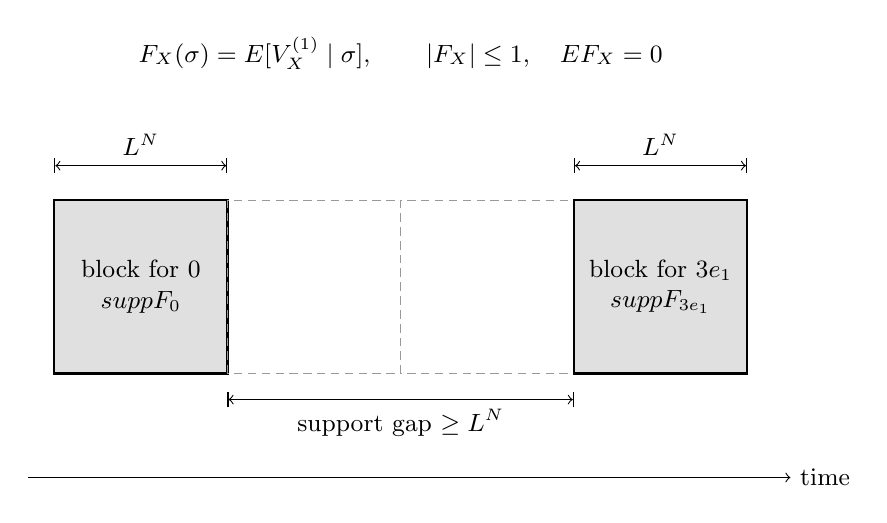
\begin{tikzpicture}[x=2.2cm,y=2.2cm,font=\small]
    \draw[fill=black!12,thick] (0,0) rectangle (1,1);
    \draw[densely dashed,black!40] (1,0) rectangle (2,1);
    \draw[densely dashed,black!40] (2,0) rectangle (3,1);
    \draw[fill=black!12,thick] (3,0) rectangle (4,1);
    \node[align=center] at (0.5,0.5) {block for $0$\\$\operatorname{supp} F_0$};
    \node[align=center] at (3.5,0.5)
      {block for $3e_1$\\$\operatorname{supp} F_{3e_1}$};

    \draw[|<->|] (0,1.2) -- (1,1.2);
    \node[above] at (0.5,1.2) {$L^N$};
    \draw[|<->|] (3,1.2) -- (4,1.2);
    \node[above] at (3.5,1.2) {$L^N$};
    \draw[|<->|] (1,-0.15) -- (3,-0.15);
    \node[below] at (2,-0.15) {support gap $\ge L^N$};
    \draw[->] (-0.15,-0.6) -- (4.25,-0.6);
    \node[anchor=west] at (4.25,-0.6) {time};

    \node at (2,1.85)
      {$\displaystyle F_X(\sigma)=\mathbb E[V_X^{(1)}\mid\sigma],
       \qquad |F_X|\le1,\quad \mathbb E F_X=0$};
  \end{tikzpicture}\par\medskip
  \caption{Pulling terminal observables back to the original lattice.
  Each displayed support lies within an ancestral block of side $L^N$.
  The auxiliary block variables are independent between disjoint
  ancestral blocks conditional on the original spins, so
  $\mathbb E[F_0F_{3e_1}]=\mathbb E[V_0^{(1)}V_{3e_1}^{(1)}]$.
  Alignment bounds this correlation below by $1/8$; the full transfer
  gap bounds it above by the exponential of minus the gap times $L^N$.
  No independence of the two pulled-back observables is asserted.}
  \label{fig:block-supports}
\end{figure}


\begin{proof}[Completion of Theorem~\ref{thm:main}]
Theorem~\ref{thm:preliminary} gives existence and uniqueness of the
periodic local limit. Proposition~\ref{rg:admission} supplies all
required trajectories and covers every sufficiently large bare
coupling. Theorem~\ref{thm:lower} and Proposition~\ref{prop:upper}
give the two bounds in depth units. Proposition~\ref{prop:calibration}
converts them to \eqref{eq:target}. Every choice of constants was made
before the final depth $N$.
\end{proof}
